\documentclass[a4paper,11pt,reqno]{amsart}

% --------------------------------------------------------
% Packages
% --------------------------------------------------------
\usepackage[utf8]{inputenc}
\usepackage{amsmath,amsfonts,amssymb,amsthm,mathrsfs,bm}
\usepackage[margin=0.95in]{geometry}
\usepackage{color}
\usepackage[dvipsnames]{xcolor}
\usepackage{mathtools,graphicx}
\usepackage{tcolorbox}
\usepackage{listings}
\usepackage{textcomp}
\usepackage{units}
\usepackage{hyperref}
\usepackage{float}
\usepackage{fancyhdr}
\usepackage{subfigure} % 支持多图
\usepackage{cite}
\usepackage{url} % bibTex支持引用网页

% --------------------------------------------------------
% Custom Colours
% --------------------------------------------------------
\definecolor{CommentGreen}{rgb}{0.0,0.4,0.0}
\definecolor{Background}{rgb}{0.9,1.0,0.85}
\definecolor{lrow}{rgb}{0.914,0.918,0.922}
\definecolor{drow}{rgb}{0.725,0.745,0.769}


% --------------------------------------------------------
% Typesetting Python code
% --------------------------------------------------------
\lstloadlanguages{Python}%
\lstset{
    language=Python, upquote=true, frame=single,
    basicstyle=\small\ttfamily,
    backgroundcolor=\color{yellow!30},
    keywordstyle=[1]\color{NavyBlue}\bfseries,
    keywordstyle=[2]\color{RubineRed},
    keywordstyle=[3]\color{orange!90}\bfseries,
    keywordstyle=[4]\color{Green!90}\bfseries,
    identifierstyle=,
    commentstyle=\usefont{T1}{pcr}{m}{sl}\color{MidnightBlue}\small,
    stringstyle=\color{purple},
    showstringspaces=false, tabsize=4, morekeywords={import,as},
    morekeywords=[2]{args,__init__},
    morekeywords=[3]{@property},
    morekeywords=[4]{self},
    morecomment=[l][\color{blue}]{...},
    numbers=none, firstnumber=1,
    numberstyle=\tiny\color{blue},
    stepnumber=1, xleftmargin=10pt, xrightmargin=10pt
}

\synctex=1

\hypersetup{
    unicode=false, pdftoolbar=true, 
    pdfmenubar=true, pdffitwindow=false, pdfstartview={FitH}, 
    pdftitle={ELE8088 Coursework}, pdfauthor={Z. Zhang},
    pdfsubject={ELE8088 coursework}, pdfcreator={Z. Zhang},
    pdfproducer={ELE8088}, pdfnewwindow=true,
    colorlinks=true, linkcolor=red,
    citecolor=blue, filecolor=magenta, urlcolor=cyan
}

% --------------------------------------------------------
% CUSTOM COMMANDS
% --------------------------------------------------------
\newcommand{\iu}{{\mathrm{i}\mkern1mu}}
\newcommand{\R}{{\rm I\!R}}
\newcommand{\N}{{\rm I\!N}}
\newcommand{\E}{{\rm I\!E}}
\newcommand{\C}{\mathbb{C}}
\newcommand{\dd}{\mathrm{d}}
\newcommand{\tran}{\intercal}
\DeclareMathOperator{\Var}{Var}
\DeclareMathOperator*{\minimise}{Minimise}
\newcommand{\smallmat}[1]{\left[ \begin{smallmatrix}#1 \end{smallmatrix} \right]}
\newcommand{\smallplus}{{\scriptscriptstyle +}}
\newcommand{\Spp}{\mathbb{S}_{\smallplus\smallplus}}
\newcommand{\Sp}{\mathbb{S}_{\smallplus}}
\newcommand{\prob}{\mathrm{P}}
\DeclareUnicodeCharacter{2212}{-}
\pagestyle{fancy}
\cfoot{\thepage} % 这条语句可以让页码出现在下方
\renewcommand\headrulewidth{0pt} % 取消页眉线
\setlength{\footskip}{25pt} % 设置页码与正文的距离
\setlength{\headheight}{13.0pt}
\addtolength{\topmargin}{-5.0pt}

% --------------------------------------------------------
% Beginning of your document
% --------------------------------------------------------
\begin{document}
\thispagestyle{fancy} % 令fancy对当前页(首页)生效
\cfoot{\thepage} % 这条语句可以让页码出现在下方
\textsc{
    \vspace{-2cm}
    \begin{center}
        \center\LARGE Queen's University Belfast \\[0.5cm]
        \Large ELE8088: Control \& Estimation Theory \\[0.5cm]
    \end{center} 
}
\textsc{
    \vspace{-0.5cm}
    \begin{center}
        \small Student: Zichi Zhang \ \ \ Student Number: 40299571
    \end{center}
}

% --------------------------------------------------------
% Section 1: Lab I - Assignment
% --------------------------------------------------------
\vspace{0.2cm}
\begin{center}
\section*{\Large Lab I - Assignment}
\end{center}

% Subsection: Optimisation problem
% ^^^^^^^^^^^^^^^^^^^^^^^^^^^
\subsection*{Question 1 [Optimisation problem]}\label{sec:q1}
(i)This paper chooses the machine epsilon \cite{ali_m-zero} to be a reasonable threshold, $\epsilon>0$, 
below which a number is considered to be practically zero. 
That is, $x$ is considered to be (practically) equal to zero 
if $\|x\|<\epsilon $. The Python code is: \href{https://github.com/Gczmy/ELE8088/blob/main/Lab1/Python_code/Question1/Question1.py}{Question 1}.
The figure of $\mathrm{sp}(x^{\star}(\mu))$ against $\mu$ 
for $0 \leq \mu \leq \mu_{\mathrm{max}}$ is shown below 
as Figure \ref{fig:q1_i}:
\vspace{-0.2cm}
\begin{figure}[H]
    \centering
    \includegraphics[width=0.7\textwidth]{figures/q1_i.eps}
    \caption{$\mathrm{sp}(x^{\star}(\mu))$ against $\mu$ for $0 \leq \mu \leq \mu_{\mathrm{max}}$}
    \label{fig:q1_i}
\end{figure}

(ii)The figure of $\left\lVert Ax^{\star}(\mu) - b\right\rVert$ against $\mu$ for $0 \leq \mu \leq \mu_{\mathrm{max}}$ is shown below as Figure \ref{fig:q1_ii}:
\begin{figure}[H]
    \centering
    \includegraphics[width=0.7\textwidth]{figures/q1_ii.eps}
    \caption{$\left\lVert Ax^{\star}(\mu) - b\right\rVert$ against $\mu$ for $0 \leq \mu \leq \mu_{\mathrm{max}}$}
    \label{fig:q1_ii}
\end{figure}

(iii)
The Figure \ref{fig:q1_i} shows that the the sparsness of $x^{\star}(\mu)$ increases rapidly with $\mu$ increasing in the beginning, and when $\mu$ more than a value which is approximately 8, the $\mathrm{sp}(x^{\star}(\mu))$ increases very slowly.
And the Figure \ref{fig:q1_ii} shows that the $\left\lVert Ax^{\star}(\mu) - b\right\rVert$ and $\mu$ can be approximately regarded as a linear relationship.

% Subsection: IHOCP and DARE
% ^^^^^^^^^^^^^^^^^^^^^^^^^^^
\subsection*{Question 2 [IHOCP and DARE]}\label{sec:q2}
(i)The Python code is: \href{https://github.com/Gczmy/ELE8088/blob/main/Lab1/Python_code/Question2/Question2.py}{Question 2}. 
$P_t$ for $t\in\N_{[1,5]}$ is shown below as $P_1$, $P_2$, $P_3$, $P_4$ and $P_5$:
$$\begin{aligned}
    P_1 &=
    \begin{bmatrix}
        3.48006722 & 0.42287465 \\
        0.42287465 & 3.72528667
    \end{bmatrix}, 
    \ \ \ P_2 =
    \begin{bmatrix}
        10.78513153 & 1.63773992 \\
        1.63773992 & 9.60377259
    \end{bmatrix},
    \\
    P_3 &=
    \begin{bmatrix}
        27.12835962 & 5.93967313 \\
        5.93967313 & 24.97062138
    \end{bmatrix}, 
    P_4 =
    \begin{bmatrix}
        62.63517376 & 10.22520071 \\
        10.22520071 & 53.7344441
    \end{bmatrix},
    \\
    P_5 &=
    \begin{bmatrix}
        109.29093751 & 5.18670927 \\
        5.18670927 & 112.97575136
    \end{bmatrix}.
    \notag
\end{aligned}$$

(ii)Yes, if $N$ is large enough, $P_N$ is approximately equal to a matrix $P$ that solves DARE.
We can let $N=50$, thus
\begin{equation}
    P_N =
    \begin{bmatrix}
        3052.97899665 & -4621.98828315 \\
        -4621.98828315 & 7588.73677777
    \end{bmatrix}
    \notag
\end{equation}
A matrix $P$ that solves DARE:
\begin{equation}
    P =
    \begin{bmatrix}
        3052.97899664 & -4621.98828313 \\
        -4621.98828313 & 7588.73677774
    \end{bmatrix}
    \notag
\end{equation}
(iii)The figure of $P_{N,1,1}$, $P_{N,1,2}$ and $P_{N,2,2}$ against $N$ is shown below as Figure \ref{fig:q2_iii}:
\begin{figure}[H]
    \centering
    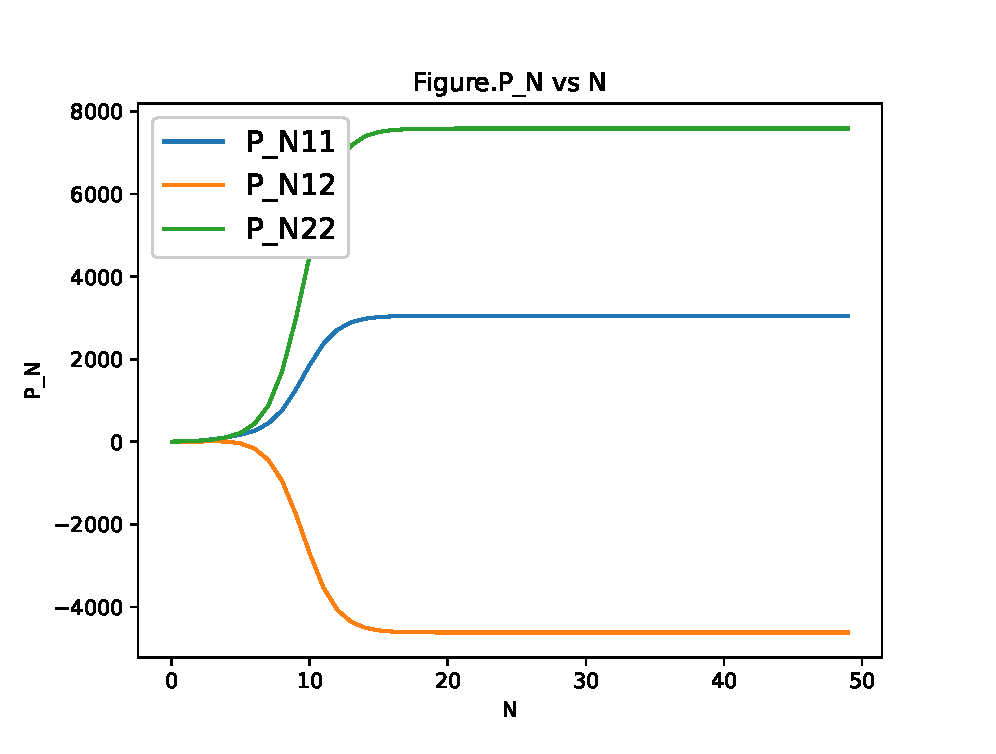
\includegraphics[width=0.7\textwidth]{figures/q2_iii.eps}
    \caption{$P_{N,1,1}$, $P_{N,1,2}$ and $P_{N,2,2}$ against $N$}
    \label{fig:q2_iii}
\end{figure}
The Figure \ref{fig:q2_iii} shows that $P_{N,1,1}$, $P_{N,1,2}$ and $P_{N,2,2}$ converged to different values, and $P_{N,1,1}$ plus $P_{N,1,2}$ approximately equal to $P_{N,2,2}$.
\\
% Subsection: Simulations of $\kappa ^{\star}_{\infty}$-controlled system
% ^^^^^^^^^^^^^^^^^^^^^^^^^^^
\subsection*{Question 3 [Simulations of \texorpdfstring{$\kappa ^{\star}_{\infty}$}{Lg}-controlled system]}\label{sec:q3}
(i)The Python code is: \href{https://github.com/Gczmy/ELE8088/blob/main/Lab1/Python_code/Question3/Question3.py}{Question 3}. We can solve the discrete-time algebraic Riccati equation and
determine an optimal stationary control law, $\kappa^{\star}_{\infty}=Kx$ (i.e., determine $K$). $K$ is shown below:
\begin{equation}
    K =
    \begin{bmatrix}
        2.92322706 & -8.71230855
    \end{bmatrix}
    \notag
\end{equation}
\\
(ii)
This paper chooses $x_0 = \begin{bmatrix} 19 & -2 \end{bmatrix}^{\tran}$ as the initial state. The figure of the states against time is shown below as Figure \ref{fig:q3_ii_states} 
and the figure of the control actions against time is shown below as Figure \ref{fig:q3_ii_control_actions}:
\begin{figure}[H]
    \centering
    \vspace{-0.35cm}
    \subfigtopskip=2pt
    \subfigbottomskip=2pt
    \subfigcapskip=-5pt
    \subfigure[States against time]{
        \label{fig:q3_ii_states}
        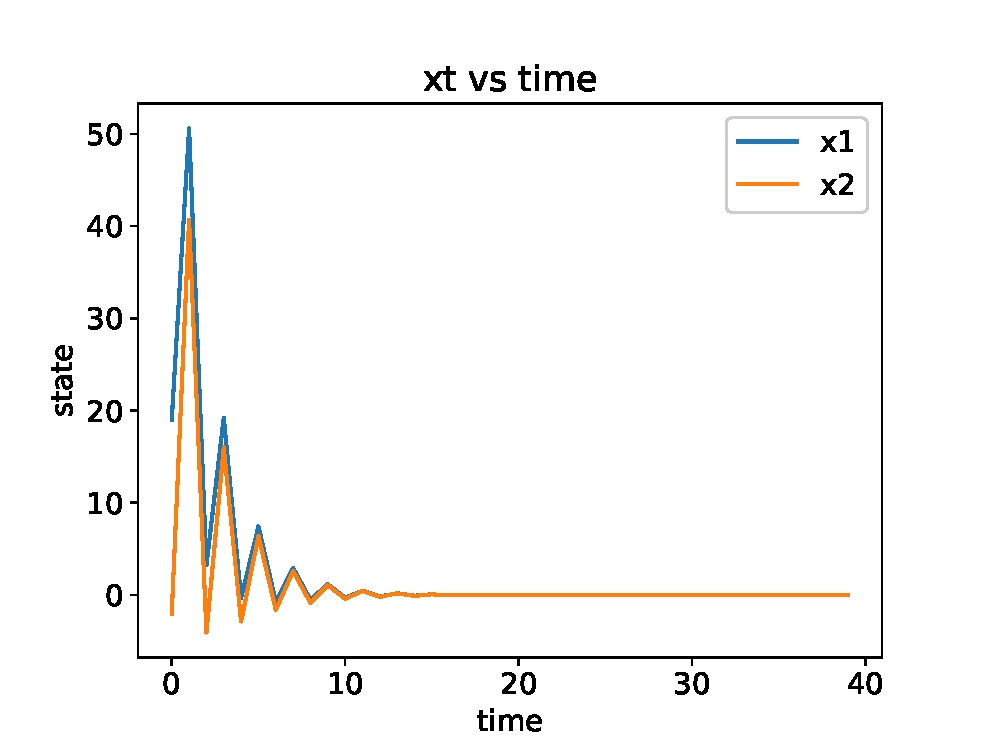
\includegraphics[width=0.45\linewidth]{figures/q3_ii_states.eps}}
    \quad
    \subfigure[Control actions against time]{
        \label{fig:q3_ii_control_actions}
        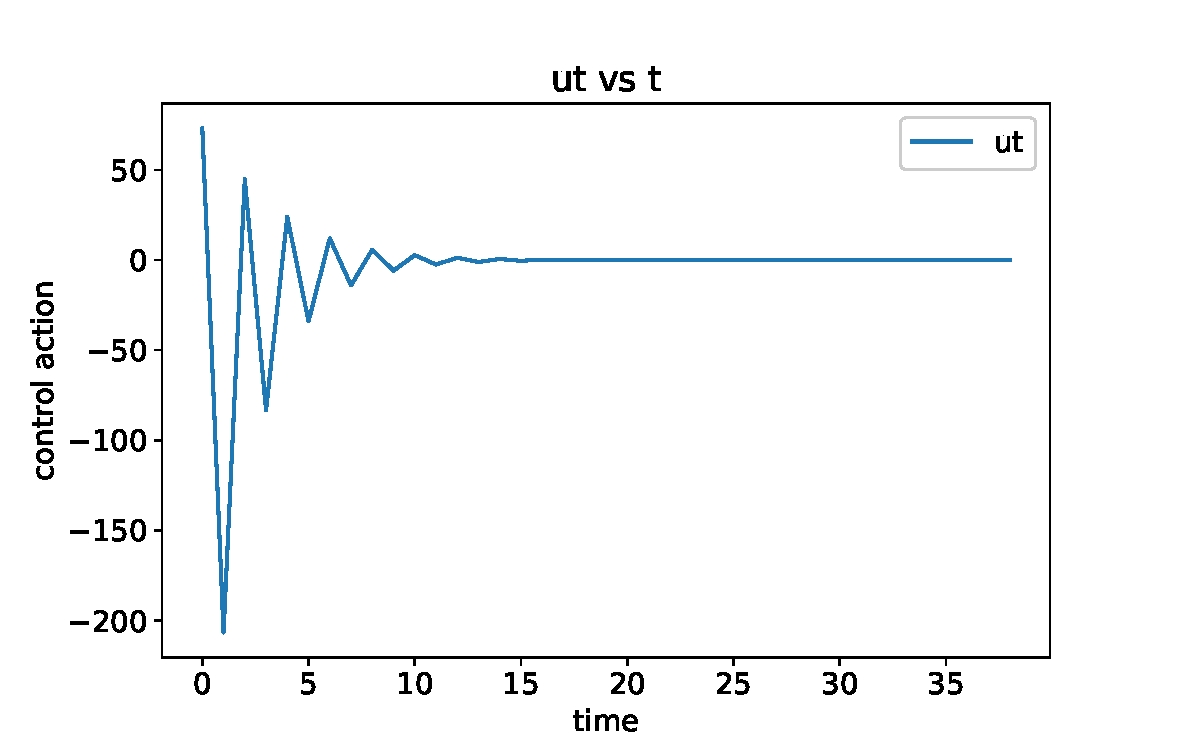
\includegraphics[width=0.45\linewidth]{figures/q3_ii_control_actions.eps}}
    \caption{States and control actions against time}
    \label{fig:q3_ii}
\end{figure}
(iii)The figure of $V^{\star}_{\infty}(x_t) $ against $t$ is shown below as Figure \ref{fig:q3_iii}:
\begin{figure}[H]
    \centering
    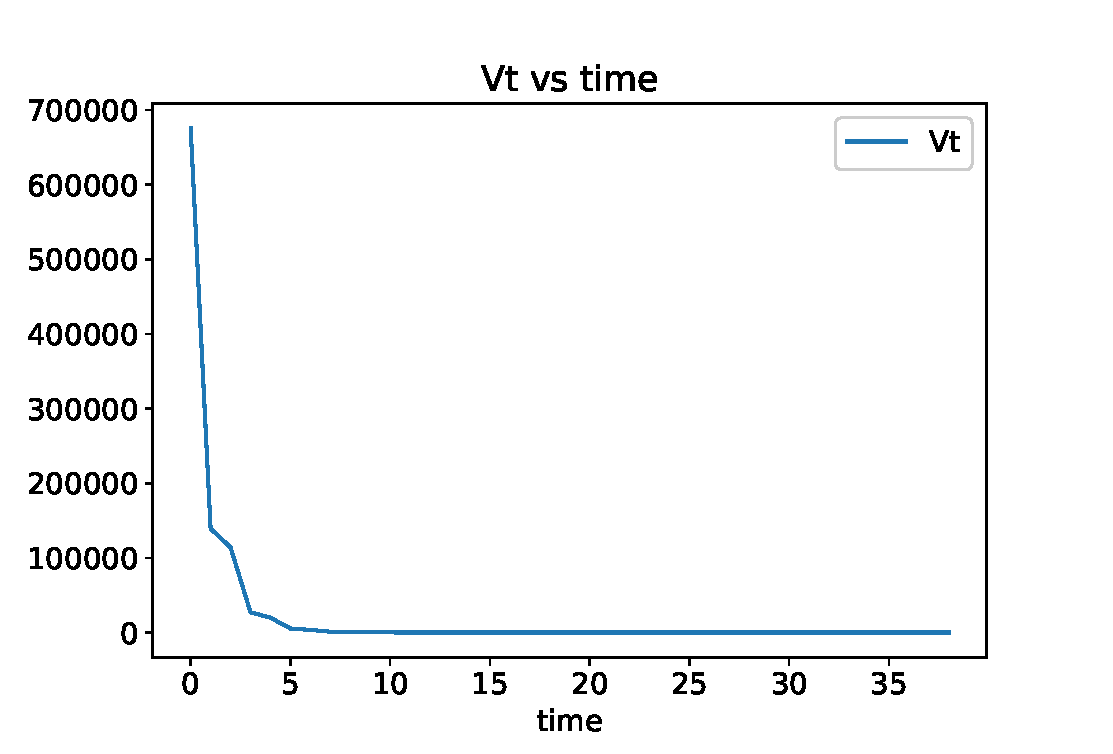
\includegraphics[width=0.7\textwidth]{figures/q3_iii.eps}
    \caption{$V^{\star}_{\infty}(x_t) $ against $t$}
    \label{fig:q3_iii}
\end{figure}

% Subsection: MPC design and simulations
% ^^^^^^^^^^^^^^^^^^^^^^^^^^^
\subsection*{Question 4 [MPC design and simulations]}\label{sec:q4}
(i)The Python code is: \href{https://github.com/Gczmy/ELE8088/blob/main/Lab1/Python_code/Question4/Question4_i%26ii.py}{Question 4 i\&ii}. 
This paper chooses $x_0 = \begin{bmatrix} 0.01 & 0.04 \end{bmatrix}^{\tran}$ as the initial state. The figure of states $x_t$ against time for the MPC-controlled system is shown below as Figure \ref{fig:q4_i_states} 
and the figure of control actions $u_t$ against time for the MPC-controlled system is shown below as Figure \ref{fig:q4_i_control_actions}:
\begin{figure}[H]
    \centering
    \vspace{-0.35cm}
    \subfigtopskip=2pt
    \subfigbottomskip=2pt
    \subfigcapskip=-5pt
    \subfigure[States against time]{
        \label{fig:q4_i_states}
        \includegraphics[width=0.45\linewidth]{figures/q4_i_states.eps}}
    \quad
    \subfigure[Control actions against time]{
        \label{fig:q4_i_control_actions}
        \includegraphics[width=0.45\linewidth]{figures/q4_i_control_actions.eps}}
    \caption{States and control actions against time}
    \label{fig:q4_i}
\end{figure}
(ii)
The figure of $V^{\star}_N(x)$ against time for the MPC-controlled system is shown below as Figure \ref{fig:q4_ii}:
\begin{figure}[H]
    \centering
    \includegraphics[width=0.7\textwidth]{figures/q4_ii.eps}
    \caption{$V^{\star}_{N}(x_t)$ against $t$}
    \label{fig:q4_ii}
\end{figure}
(iii)The Python code is: \href{https://github.com/Gczmy/ELE8088/blob/main/Lab1/Python_code/Question4/Question4_iii.py}{Question 4 iii}. 
The finite horizon optimal control problem:
\begin{subequations}
    \begin{align}
        \mathbb{P}_N(x): \minimise_{x\in \R^n}\sum_{t=0}^{N-1}\, 
        & \textstyle\frac{1}{2}\left(x_t^{\tran}Qx_t+Ru^2_t\right)+\frac{1}{2}x_N^{\tran}Px_N,
        \\
        \text{subject to: }\,
        & x_{t+1} = A x_t + B u_t, t\in\N_{[0, N-1]}, \label{formula:q4iii_1b}
        \\
        & x^{\tran}Px\leq \alpha,
        \\
        & x_{\mathrm{min}}\leq x_t\leq x_{\mathrm{max}}, t \in \N_{[1, N]},
        \\
        & u_{\mathrm{min}}\leq u_t\leq u_{\mathrm{max}}, t \in \N_{[0, N-1]},
        \\
        & x_{0} = x.
    \end{align}
\end{subequations}
We want to limit the magnitude of the successive changes of the state; in other
words, we need to limit the velocity of the state. In particular, we want to impose the constraint:
$$\|x_{t+1}-x_t\|_{\infty}\leq 0.05$$
We can use the formula (Equation \ref{formula:q4iii_1b}): $x_{t+1} = A x_t + B u_t, t\in\N_{[0, N-1]}$, thus, we can get



% $$\|(A-I)x_t+Bu_t\|_{\infty}\leq 0.05$$
% $$\|A\|_{\infty}=\max_{1\leq i\leq m}\sum^n_{j=1}\left\lvert a_{ij}\right\rvert$$ where $A\in \R^{m\times n}$
% \begin{equation}
%     A =
%     \begin{bmatrix}
%         0.9  & 1.5 \\
%         -1.3 & -0.7
%     \end{bmatrix}, 
%     B =
%     \begin{bmatrix}
%         0.5 \\
%         0.2
%     \end{bmatrix}
%     \notag
% \end{equation}
% \begin{equation}
%     A-I =
%     \begin{bmatrix}
%         -0.1 & 1.5 \\
%         -1.3 & -1.7
%     \end{bmatrix}
%     \notag
% \end{equation}
% \begin{equation}
%     (A-I)x_t+Bu_t =
%     \begin{bmatrix}
%         -0.1 & 1.5 \\
%         -1.3 & -1.7
%     \end{bmatrix}
%     \begin{bmatrix}
%         x_{t,1} \\
%         x_{t,2}
%     \end{bmatrix}
%     +
%     \begin{bmatrix}
%         0.5 \\
%         0.2
%     \end{bmatrix}
%     \begin{bmatrix}
%         u_{t,1} \\
%         u_{t,2}
%     \end{bmatrix}
%     =
%     \begin{bmatrix}
%         -0.1x_{t,1}+1.5x_{t,2}+0.5u_{t,1}+0.5u_{t,2} \\
%         -1.3x_{t,1}-1.7x_{t,2}+0.2u_{t,1}+0.2u_{t,2}
%     \end{bmatrix}
%     \notag
% \end{equation}
% \begin{equation}
%     \max_{1\leq i\leq 2}\left\lvert 
%     \begin{bmatrix}
%         -0.1x_{t,1}+1.5x_{t,2}+0.5u_{t,1}+0.5u_{t,2} \\
%         -1.3x_{t,1}-1.7x_{t,2}+0.2u_{t,1}+0.2u_{t,2}
%     \end{bmatrix}
%     \right\rvert\leq 0.05, t\in \N_{[0,N-1]}
% \notag
% \end{equation}
% \begin{equation}
%     -0.05\leq
%     \max_{1\leq i\leq 2} 
%     \begin{bmatrix}
%         -0.1x_{t,1}+1.5x_{t,2}+0.5u_{t,1}+0.5u_{t,2} \\
%         -1.3x_{t,1}-1.7x_{t,2}+0.2u_{t,1}+0.2u_{t,2}
%     \end{bmatrix}
%     \leq 0.05, t\in \N_{[0,N-1]}
% \notag
% \end{equation}
% \begin{equation}
%     \begin{cases}
%         -0.05\leq -0.1x_{t,1}+1.5x_{t,2}+0.5u_{t,1}+0.5u_{t,2}\leq 0.05 \\
%         -0.05\leq -1.3x_{t,1}-1.7x_{t,2}+0.2u_{t,1}+0.2u_{t,2}\leq 0.05, t\in \N_{[0,N-1]}
%     \end{cases}
%     \notag
% \end{equation}


\begin{equation}
    \|(A-I)x_t+Bu_t\|_{\infty}\leq 0.05, t\in \N_{[0,N-1]}
\notag
\end{equation}
Then we can modify the problem $\mathbb{P}_N(x)$ (Equation (1)) and update the constraints of the problem to achieve this.
The finite horizon optimal control problem after modifying:
\begin{subequations}
    \begin{align}
        \mathbb{P}_N(x): \minimise_{x\in \R^n}\sum_{t=0}^{N-1}\,
        & \textstyle\frac{1}{2}\left(x_t^{\tran}Qx_t+Ru^2_t\right)+\frac{1}{2}x_N^{\tran}Px_N,
        \\
        \text{subject to: }\,
        & x_{t+1} = A x_t + B u_t, t\in\N_{[0, N-1]},
        \\
        & \|(A-I)x_t+Bu_t\|_{\infty}\leq 0.05, t\in \N_{[0,N-1]},
        \\
        & x_{\mathrm{min}}\leq x_t\leq x_{\mathrm{max}}, t \in \N_{[1, N]},
        \\
        & u_{\mathrm{min}}\leq u_t\leq u_{\mathrm{max}}, t \in \N_{[0, N-1]},
        \\
        & x_{0} = x.
    \end{align}
\end{subequations}

Then, we can simulate it by Python. This paper chooses $x_0 = \begin{bmatrix} 0.01 & 0.04 \end{bmatrix}^{\tran}$ as the initial state. The figure of states $x_t$ against time is shown below as Figure \ref{fig:q4_iii_states}
and the figure of control actions $u_t$ against time for the MPC-controlled system is shown below as Figure \ref{fig:q4_iii_control_actions}:
\begin{figure}[H]
    \centering
    \vspace{-0.35cm}
    \subfigtopskip=2pt
    \subfigbottomskip=2pt
    \subfigcapskip=-5pt
    \subfigure[States against time]{
        \label{fig:q4_iii_states}
        \includegraphics[width=0.45\linewidth]{figures/q4_iii_states.eps}}
    \quad
    \subfigure[Control actions against time]{
        \label{fig:q4_iii_control_actions}
        \includegraphics[width=0.45\linewidth]{figures/q4_iii_control_actions.eps}}
    \caption{States and control actions against time}
    \label{fig:q4_iii}
\end{figure}
The figure of $V^{\star}_{\infty}(x_t) $ against $t$ is shown below as Figure \ref{fig:q4_iii_cost}:
\begin{figure}[H]
    \centering
    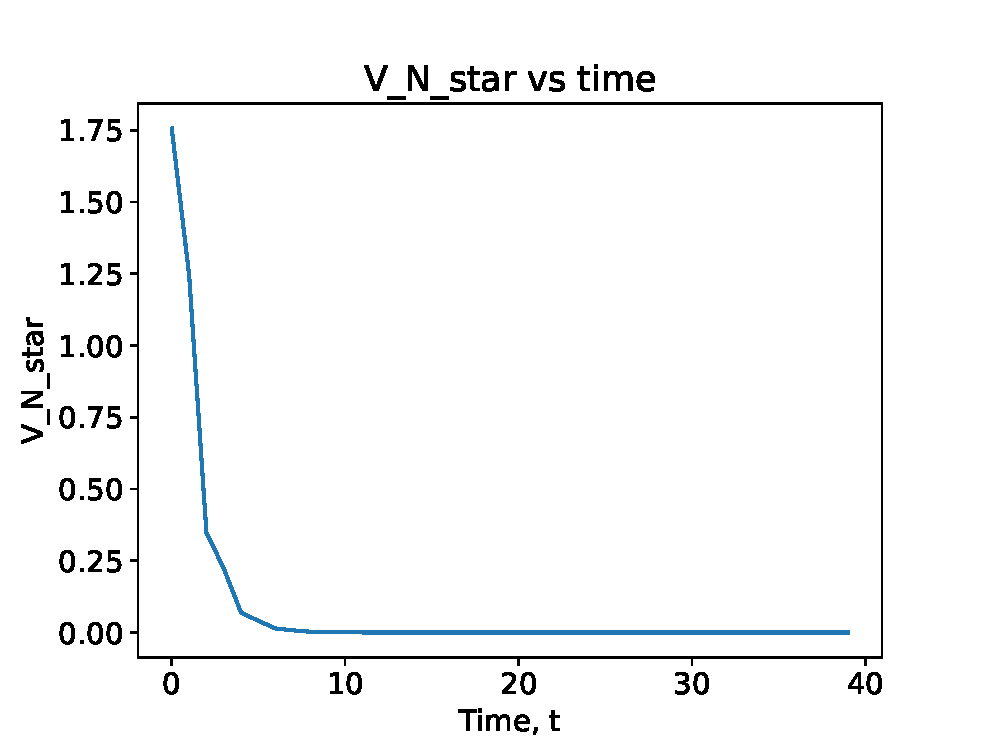
\includegraphics[width=0.7\textwidth]{figures/q4_iii_cost.eps}
    \caption{$V^{\star}_{\infty}(x_t) $ against $t$}
    \label{fig:q4_iii_cost}
\end{figure}


\bibliographystyle{IEEEtran}
\bibliography{References}
\end{document}
